% Template for Cogsci submission with R Markdown

% Stuff changed from original Markdown PLOS Template
\documentclass[10pt, letterpaper]{article}

\usepackage{cogsci}


\title{Not so opaque after all: Conventions formed in reference games
are mostly understandable to outsiders}

\cogscifinalcopy

\author{{\large \bf Veronica Boyce (vboyce@stanford.edu)} \\ Department of Psychology \\ Stanford University \And {\large \bf Ben Prystawski (benpry@stanford.edu)} \\Department of Psychology \\ Stanford University \AND {\large \bf Alvin Wei Ming Tan (tanawm@stanford.edu)} \\ Department of Psychology \\ Stanford University \And {\large \bf Michael C. Frank (mcfrank@stanford.edu)} \\ Department of Psychology \\ Stanford University}


\begin{document}

\maketitle

\begin{abstract}
In-groups can create conventionalized language, but this jargon may be
understandable to those outside the group. The formation of temporary
linguistic conventions between individuals is often studied in iterated
reference games, where over repeated reference to the same targets, a
describer-matcher pair establishes conventional shorthand names for
targets. One angle on convention formation is how understandable
referring expressions from different stages are to outsiders. Here, we
take an outside angle on understanding convention formation, using
experiments with naive matchers and computational models to assess the
opacity of descriptions from iterated reference games. Both human
matchers and the computational model are well above chance accuracy,
with variation in performance primarily driven by the target image
rather than where or when the description came from. TODO wrap up
sentence

\textbf{Keywords:}
TODO keywords
\end{abstract}

\section{Introduction}\label{introduction}

TODO need an actually good hook/intro We can often understand what
people are saying even when we are not the intended audience. From
snippets of overheard conversation, we can construct what is going on
well enough to understand it.

We can understand more than we produce; for instance, even if I would
call the object a ``water fountain'' I can understand what another
person means when they say ``bubbler''.

While some different terms are conventionally set and shared among large
groups of people as language, or regional dialect, or field specific
jargon, temporary conventions can be formed with smaller groups of
people as a matter of conversational necessity to have a term to refer
to a thing with.

This formation of temporary linguistic conventions between individuals
is often studied in iterated reference games. In these games, a
describer tells their partner or partners how to sort or match a series
of abstract images (Clark \& Wilkes-Gibbs, 1986; Hawkins et al., 2020).
Over repeated rounds, the same set of images are referred to repeatedly
and pairs usually develop agreed upon nicknames for the target images.
These nicknames are often partner-specific, in that different pairs
develop different nicknames for the same targets. Describers seem to
expect that naive partners will need more elaborated descriptions. The
same describer may use different terms for the target image if their
partner changes, for instance going back to more elaborated terms with a
new partner, even if that partner was present in the room (Wilkes-Gibbs
\& Clark, 1992; Yoon \& Brown-Schmidt, 2018). {[}OTHER THINGS WE COULD
CITE{]}

How strongly partner-specific are the conventions created in iterated
reference games? Are they merely created for in the context of the
partnership, or are they also only or mostly interpretable to those who
were part of the in-group? The partner-specifity of conversational pacts
is often studied by looking at how the pacts are created, and how
utterances change over the course of games (Boyce et al., 2024; Hawkins
et al., 2020). Another angle on convention formation is to look at the
degree of arbitrariness by seeing how understandable the conventions are
to others who were not part of the interaction that originated the
convention. A more arbitrary convention should be harder to understand.

Asking naive matchers to interpret utterances produced during iterated
reference games thus can provide an additional perspective by
determining how the features of the utterances and the conditions they
were produced under affect how opaque they are, and provide empirical
tests of whether descriptions become more opaque over the course of the
reference game.

Some prior work has investigated how well naive matchers can understand
the descriptions produced in the course of an iterated reference game,
with a focus on how the presence or absence of the shared history
affects understanding.

Murfitt \& McAllister (2001) had 8 participants describe tangram shapes
in an iterated matching game with or without a partner, and then played
the recorded descriptions to new listeners either in round order or in
reverse round order. Naive listeners were more accurate when the heard
descriptions in the order they were produced rather than the reverse
order. Murfitt \& McAllister (2001) also looked at various features of
the descriptions such as utterance length and definiteness, but none of
these features significantly predicted accuracy. TODO look up actual
accuracy rates?

Schober \& Clark (1989) had pairs of participants repeatedly arrange
arrays of 12 tangram figures from an overall pool of 16 figures. The
in-game matchers had mean accuracies above 90\% and rising to close to
100\% by the 6th repetition. Naive listeners who heard the entire game
in order, either live, as it was played, or on recording, had accuracies
that started around 75\% and rose to 90\%. Matchers who listened to
recordings starting in the 3rd round of the round of the game did worse,
with initial accuracies around 55\% that rose slowly to 70\%. TODO
double check if they report numbers of if we're just eyeballing the
plots

In an iterated reference game using drawing (rather than text) as the
communication modality, Hawkins et al. (2023) compared the accuracy of
matchers who were part of the reference game to later naive matchers in
yoked and shuffled conditions. The yoked matchers saw all the trials
from one game in the same order as they occurred; the shuffled matchers
saw trials sampled from 10 games but ordered based on when in the games
they occurred. In-game matchers were more accurate overall (88\% on
4-way choice) than yoked matchers (75\%) who were in turn more accurate
than shuffled matchers (TODO I don't think this number of
reported\ldots). Over the course of trials, both in-game and yoked
matchers showed steeper improvement in accuracy than shuffled matchers.

While ``overhearers'' have worse accuracy than in-game matchers, their
performance is still far above chance, suggesting that at least some of
the content of referential pacts is accessible. In fact, even when pairs
of participants try to obfuscate their meaning to match images with each
other but not an overhearer, an overhearing participant can still do
quite well. In Clark \& Schaefer (1987), the target matcher had an
average accuracy of 80\% rising to 95\% over repetitions (on a set of 8
targets) while overhears had an average accuracy of 45\%, despite the
goal being to prevent the overhearers comprehension. TODO maybe don't
include

Across these studies, recieving more context from one interaction, and
in particular, having that context be in order, is beneficial to
matchers. Except for the shuffled condition of Hawkins et al. (2023),
these studies do not address how well matchers do at isolated
descriptions from different games and points in the game.

The outside perspective on iterated reference games has also been used
to disentangle comprehension and production abilities, by providing
descriptions from the first and last rounds of a parent-child iterated
reference game to adults and children serving as naive matchers (Leung
et al., 2024). They found no significant difference in how
comprehensible early and late desciptions were to naive matchers. TODO
look up actual accuracy rates relative to live!

\subsection{ALvin gets to write computational intro
here}\label{alvin-gets-to-write-computational-intro-here}

One way to conceptualize the opacity of a referring expression is by
considering the semantic distance between the signifier and the
referent. Under the assumption of a modality-independent global
semantics (i.e., not conditioned by partner-specific meaning),
expressions that are transparent have signifiers and referents that are
semantically close, such that any member of the sociolinguistic
community sharing the global semantics should be able to identify the
appropriate referent given the signifier. In contrast, expressions that
are opaque have signifiers and referents that are semantically distant,
such that the relations between them are more arbitrary and inaccessible
to the general community without the formation of additional conventions
(which may be partner- or group-specific).

Assessing opacity thus requires us to have a measure of
modality-independent global semantics. Such semantics are difficult to
directly obtain for humans, since we rarely have explicit semantic
formulations of the stimuli we encounter, and much less formulations
which are unifed across multiple modalities. However, the ability of a
naïve comprehender to understand a referring expression that is
presented without context provides a proxy measure, since the
comprehender's judgements are not conditioned on any context-specific
conventions. Thus, prior studies on naïve matchers provide one approach
to estimating the opacity of the utterances produced in reference games.

Another possible measure of modality-independent global semantics is
computational in origin. Computational methods have enabled the
projection of various stimuli (including image and text stimuli) into
embeddings in high-dimensional spaces; these embeddings have
demonstrated properties which suggest that they are reasonable
approximations of humans' semantic spaces, including similarity in
representational geometries (e.g., Grand et al., 2022; Muttenthaler \&
Hebart, 2021). Indeed, embeddings from neural network models have been
used as a form of semantics in a range of reference game scenarios
(e.g., Gul \& Artzi, 2024; Ji et al., 2022; Kang et al., 2020; Le et
al., 2022; Ohmer et al., 2022). In particular, such embeddings can be
treated as context-independent semantic representations, since they are
not updated to account for convention formation within an iterated
reference game; hence, they can serve as a computational comparison to
human performance on a naïve matching task.

TODO some paragraph to transition back to the important questions

In the current work, we ask how does the process of convention formation
determine how easy a referential expression is for an outsider to
understand. Using reference expressions created in different games from
Boyce et al. (2024), we use both human experiments and models to assess
when and why expressions are opaque or understandable to outside
observers.

\section{Task Setup}\label{task-setup}

\subsection{Materials}\label{materials}

We draw on the corpus of reference game transcripts and results from
Boyce et al. (2024). There were all 6 round iterated reference games
using the same 12 target images, but varied in how large the groups were
(2-6 participants per group) and how ``thick'' the communication channel
between group members was. For our human experiments, we sample
different subsets of this corpus in different experiments. Within the
samples, we avoided showing participants descriptions that had swear
words or crude or sexual language. We use the entire corpus for our
computational modelling component.

\subsection{Experimental procedure}\label{experimental-procedure}

We recruited participants from Prolific (TODO criteria). Participants
were directed to the experiment, where it was explained that previously,
other participants had described these shapes to one another. They would
see a series of transcripts from the prior game, and their task was the
guess what the intended target was. On each trial participants saw the
full transcript from that trial, containing all the chat messages marked
by whether they were from the speaker or a listener (TODO confirm the
language used), except for lines that Boyce et al. (2024) had marked as
not having any referential content. Participants selected the image they
thought was the target from the tableau of 12. Participants received
feedback on whether they were right or wrong on each trial. Except when
the specific viewing order was part of the experimental manipulation, we
randomized the order of trials, subject to the constraint that the same
target could not repeat on adjacent trials.\\
The task was implemented in jsPsych. We paid participants \$10 an hour
plus a bonus of 5 cents per correct response.

\begin{CodeChunk}
\begin{figure}[t!]

{\centering 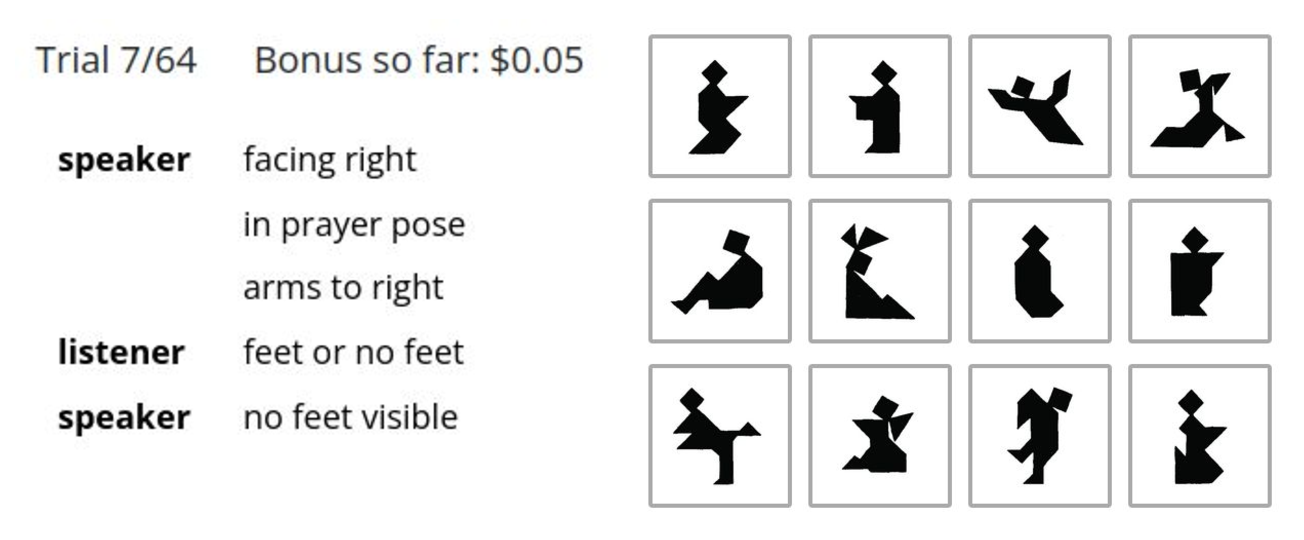
\includegraphics[width=1\linewidth]{matcher-diagram} 

}

\caption[Experimental Setup and Procedure]{Experimental Setup and Procedure. TODO \label{game}}\label{fig:interface}
\end{figure}
\end{CodeChunk}

Computational methods TODO V doesn't know how to write this QUESTION: do
we focus on mlp pre- or post- calibration?

\section{Experiment 1}\label{experiment-1}

\begin{CodeChunk}
\begin{figure}[t]

{\centering 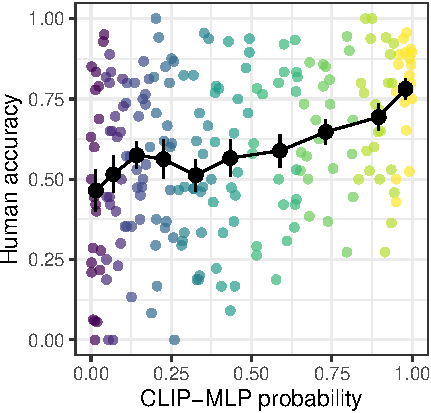
\includegraphics[width=0.7\linewidth]{figs/fig-calibration-1} 

}

\caption[Correlation between human and CLIP-MLP accuracy across deciles of CLIP-MLP accuracy]{Correlation between human and CLIP-MLP accuracy across deciles of CLIP-MLP accuracy. Colored points are individual descriptions, black line is the boostrapped mean and 95\% CI across descriptions for each decile. \label{calibration}}\label{fig:fig-calibration}
\end{figure}
\end{CodeChunk}

Our CLIP-MLP computational model was optimized for task accuracy. To
validate whether this objective also results in human-like response
patterns, we conducted a calibration experiment to determine if, for any
given utterance, the probability that the model assigns to the target
image is aligned with the probability that a naïve human matcher would
choose the target image. We hypothesized that there would be a
significant correlation between the target choice probability of the
model and the target choice probability of naïve human matchers.

\subsection{Methods}\label{methods}

We first obtained target probabilities from our CLIP-MLP model for all
utterances from Boyce et al. (2024). We then used stratified sampling to
select 217 trials by dividing model-predicted probabilities into deciles
and choosing approximately 22 utterances per decile, spanning the 12
different possible target images.

We recruited 61 participants who each saw 64 trials randomly sampled
from the 217 tested trials. On average, each trial was seen by 18
participants. This experiment was pre-registered at
\url{https://osf.io/6pv5e}.

\subsection{Results}\label{results}

We obtained human accuracies on each trial by dividing the number of
participants who correctly selected the target image by the total number
of participants who saw the trial, as shown in Figure
\ref{fig:fig-calibration}. There was a small but significant positive
correlation between model-predicted probabilities and human accuracies
(\(r\) = 0.3348057, \(p\) \textless{} .001). This result suggests that
model predictions were in fact calibrated to human response patterns,
albeit not perfectly. It is theoretically possible to use these
calibration results to project model predictions in order to better
approximate human responses; we leave this approach for future work.
Nonetheless, the observed positive correlation suggests that our
computational model was a reasonable approximation of human accuracies,
validating its use in subsequent experiments as a computational
comparison.

\section{Experiment 2}\label{experiment-2}

As a starting point for examining what makes referential expressions
more or less opaque, we had people read the descriptions from the
beginnings and ends of games. The idea of reduction and
partner-specificity would suggest that the conventionalized, later round
utterances would rely on the history of the game that naive matchers
were not privy to, and thus that late round utterances would be more
opaque and difficult to understand. On the other hand, describers gained
practice over repetitions, so later round utterances might be better at
clearly communicating the most visually salient features.

We included descriptions from games of different sizes and communication
thicknesses. In terms of group conditions, based on the patterns of
cross-game similarity in Boyce et al. (2024), we thought that smaller
and thicker games were more likely to rapidly develop ideosyncratic
conventions that would be more opaque than the less ideosyncratic
conventions from larger groups with thinner communication channels.

\subsection{Methods}\label{methods-1}

\subsubsection{Experiment 2a}\label{experiment-2a}

To establish a baseline of how well naive matchers could understand
descriptions without context, we ran a 2x2 within subjects experiment.
We drew the target transcripts from 2 and 6 player games from Experiment
1 of Boyce et al. (2024) and from the first and last (sixth) blocks of
these games. These games had medium thick communication channels. We
recruited 60 participants who each saw 60 trials (15 in each of the 4
conditions). Overall, participants saw 774 transcripts from 40 games.
This experiment was pre-registered at \url{https://osf.io/k45dr}.

\subsubsection{Experiment 2b}\label{experiment-2b}

After observing limited condition differences in experiment 2a, we ran a
second study drawing from the more extreme communication channel
thicknesses of Experiment 3 in Boyce et al. (2024). Here, we used a
2x2x2 within subjects design, drawing our transcripts from the thick and
thin, 2 and 6 person, 1st and 6th block utterances. In the thin
condition, original matchers could only contribute to the chat by
sending one of 4 emojis; as the emojis did not have referential content,
we did not include them in the transcripts shown to naive matchers. For
experiment 2b, we recruited 60 participants who each saw 64 trials (8 in
each of the 8conditions). Overall, participants saw 2392 transcripts
from 163 games. This experiment was pre-registered at
\url{https://osf.io/rdp5k}.

\begin{CodeChunk}
\begin{figure}[t]

{\centering 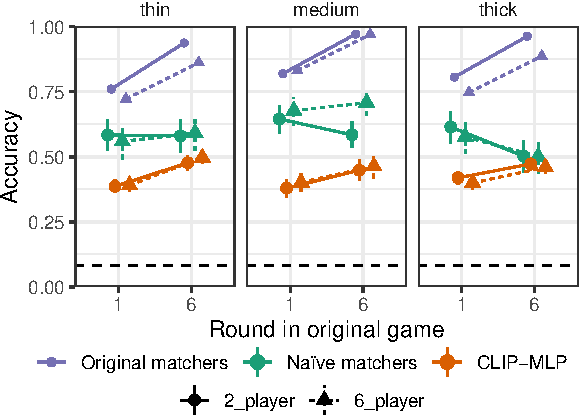
\includegraphics[width=0.9\linewidth]{figs/fig-condition-1} 

}

\caption[Accuracies for naive humans and the CLIP-MLP model for Experiment 2]{Accuracies for naive humans and the CLIP-MLP model for Experiment 2. Point estimates and 95\% CrI are predictions from the fixed effects of logistic and beta regressions. Bootstrapped mean accuracy from the original matchers is included as a ceiling, and random chance as a baseline. \label{expt2-condition}}\label{fig:fig-condition}
\end{figure}
\end{CodeChunk}

\begin{CodeChunk}
\begin{figure}[t]

{\centering 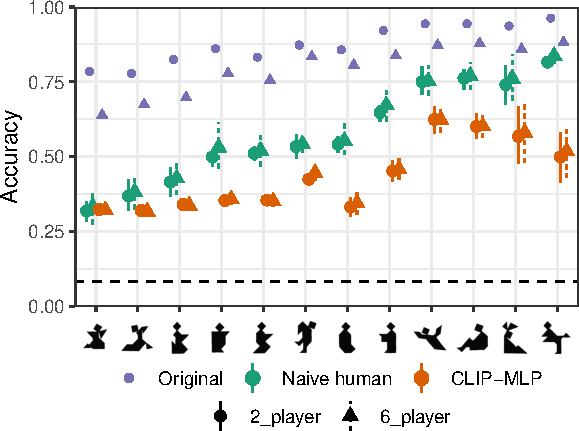
\includegraphics[width=0.9\linewidth]{figs/fig-2-1} 

}

\caption[Accuracies for naive humans and the CLIP-MLP model for Experiment 2, split out by target image]{Accuracies for naive humans and the CLIP-MLP model for Experiment 2, split out by target image. Point estimates and 95\% CI are predictions from the fixed effects and by-tangram random effects of logistic and beta regressions, bootstrapped across conditions. Bootstrapped mean accuracy from the original matchers is included as a ceiling, and random chance as a baseline. \label{expt2-tangram}}\label{fig:fig-2}
\end{figure}
\end{CodeChunk}

\subsection{Results}\label{results-1}

Our primary outcome was how accurate naive matchers would be at
selecting the correct target, and how much this would vary depending on
what game and what round the description came from.

\subsubsection{Experiment 2a}\label{experiment-2a-1}

For Experiment 2a, we ran a mixed effects logistic model of naive
matcher accuracy: correct\(\sim\) group\_size \(\times\) round~+
trial\_order~+ (group\_size \(\times\) round\textbar correct\_tangram)~+
(group\_size \(\times\) round~+ trial\_order\textbar workerid). Overall,
naive matchers were right more often than not, which was far above the
1/12 expected by random chance3 (OR: 1.93 {[}1.05, 3.62{]}. As seen in
Figure \ref{expt2-condition} middle panel, there were not large effects
of condition. Participants tended to be less accurate at descriptions
from the last round (OR of last round: 0.77 {[}0.53, 1.1{]}). There was
not a clear effect of transcripts from 6-player games (OR: 1.15 {[}0.89,
1.47{]}), but there was an interaction between round and group size (OR:
1.49 {[}1.06, 2.1{]}). Later transcripts from larger games were easier
to understand, but later transcripts from smaller games were easier to
understand. Much of the variation in accuracy was instead driven by
variation in the target images (OR of standard deviation of image
distribution: 2.66 {[}1.88, 4.52{]}. Some images were much easier to
identify as the target than others (Figure \ref{expt2-tangram}.

\subsubsection{Experiment 2b}\label{experiment-2b-1}

For Experiment 2b we ran a similar mixed effects logistic model,
consider the effects of group size, thickness, and round and their
interactions. Overall, naive matchers were above 50\% accuracy (OR: 1.81
{[}1.06, 3.08{]}). Similar to experiment 2a, there were not substantial
effects of condition. Last round descriptions had slightly lower
accuracy (OR of last round: 0.64 {[}0.47, 0.85{]}), but there was an
interaction with thickness, where thin, last round were less opaque (OR:
1.55 {[}1.02, 2.33{]}).

Again some of the uncertainty in estimating the fixed effects was driven
by the strong effects of target image (OR of SD of images: 2.25 {[}1.67,
3.59{]}).

\subsubsection{Additional Predictors}\label{additional-predictors}

As additional post-hoc predictors, we also examined the predictive value
of the accuracy of the original matchers from Boyce et al. (2024) and
the the length of the description from the original describer. In both
experiments, original accuracy was predictive of naive matcher accuracy
(Expt 2a OR: 3.38 {[}2.46, 4.7{]}, Expt 2b OR: 2.17 {[}1.7, 2.77{]}).
The log number of words in the description was not predictive in
Experiment 2a (OR: 1.05 {[}0.94, 1.17{]}), but longer descriptions were
slightly beneficial in Experiment 2b (OR: 1.1 {[}1.01, 1.2{]}).

\subsection{Model results}\label{model-results}

As a computational comparison, we looked at the CLIP-MLP model's
performance on the same descriptions. We used the probability the model
assigned as a measure of the model's accuracy, and fit a beta regression
on the descriptions from Experiment 2: correct\(\sim\) group\_size
\(\times\) thickness \(\times\) round~+ (group\_size \(\times\)
thickness \(\times\) round\textbar correct\_tangram). The CLIP-MLP model
was far above chance, but had lower accuracy than the human participants
(OR: stats\_text(acc\_mod\_mlp, 1) .

None of the fixed effects in the model were significant, and there was
wide uncertainty for all of them. There is substantial by-tangram
variation 1.58 {[}1.31, 2.15{]} and substantial by-tangram variation in
the effect of later round 1.56 {[}1.29, 2.09{]}.

As additional predictors, we checked the effect of original matcher
accuracy and the length of the description. MLP-CLIP had higher accuracy
when original matcher accuracy was higher (OR: 1.5 {[}1.33, 1.69{]}),
and the model did better on shorter descriptions (OR for log words: 0.85
{[}0.82, 0.9{]}). Long descriptions may be further from the model's
training distribution of image captions.

\subsubsection{Interim Summary}\label{interim-summary}

Overall, naive human matchers were fairly accurate overall, but less
accurate than matchers in the original game. Perhaps surprisingly, this
level of accuracy was fairly consistent across descriptions from
different times in the game and different game conditions. The largest
source of variability was from the target images; while there was some
variabiliity in accuracy by images for the original matchers, there was
substantially more variability for naive matchers.

\section{Experiment 3}\label{experiment-3}

In Experiment 2, we saw that naive matchers could understand the
descriptions fairly well, but had lower accuracy than the matchers in
the original games. There are several differences between these two,
including getting descriptions from a consistent group, getting
descriptions in order, and being a present participant during the game.
In Experiment 3, we focus on the role of context and group-specific
interaction history to tease apart some of these differences.

\subsection{Methods}\label{methods-2}

Following CITE ROBERT AND JUDY, we compared naive matchers in ``yoked''
and ``shuffled'' conditions. In the ``yoked'' condition, naive matchers
saw all the descriptions from a single game in the order they originally
occurred. In the ``shuffled'' condition, naive matchers saw all the
descriptions from a single game in a randomized order.

Because some descriptions are already pretty understandable in
isolation, we wanted to focus on the role of context in games that
showed strong group-specificity. We hand-picked 10 games from Boyce et
al. (2024) on the basis of high original matcher accuracy, strong
reduction in the length of utterances, and the use of idiosyncratic or
non-modal referring expressions. Thus, the referring expressions were
very understandable to groups who created them, but likely to be opaque
out of context.

We recruited 196 participants (99 in the yoked condition and 97 in
shuffled) who each saw all 72 trials of 1 of the 10 games. This
experiment was pre-registered at \url{https://osf.io/zqwp5}.
Participants read the transcripts in a modified self-paced reading
procedure where they uncovered the text word by word (revealed words
stayed visible); only after uncovering the entire transcript could
participants select an image. We do not analyse the word-by-word reading
data here.

\begin{CodeChunk}
\begin{figure}[t]

{\centering 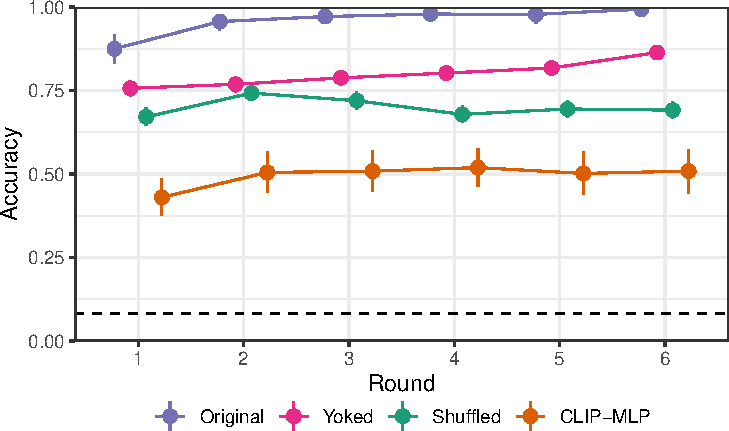
\includegraphics[width=0.9\linewidth]{figs/fig-yoked-1} 

}

\caption[Accuracies for Experiment 3]{Accuracies for Experiment 3. Error bars are bootstrapped 95\% CIs. TODO not using predictions because those fuzz out round to round differences. \label{yoked}}\label{fig:fig-yoked}
\end{figure}
\end{CodeChunk}

\subsection{Results}\label{results-2}

Our primary question of interest was how much having the conversation
history would help make later round descriptions more understandable to
participants in the yoked condition.

We compared accuracy across the yoked and shuffled conditions with a
logistic regression: correct\(\sim\) orig\_repNum \(\times\) condition~+
matcher\_trialNum~+ (1\textbar gameId)~+ (1\textbar correct\_tangram)~+
(1\textbar workerid). The descriptions were more transparent when they
were presented in a yoked order (OR: 2.2 {[}1.63, 3{]}, Figure
\ref{yoked}). In the shuffled condition, there was no main effect of
round number (OR for one round later: 0.99 {[}0.95, 1.02{]}), but there
was a marginal interaction where the benefit of the yoked condition
decreased for later rounds (OR for one round later: 0.94 {[}0.89, 1{]}).
This was offset by matchers in both conditions improving at the task
over time (OR for one trial later in matcher viewing order: 1.02
{[}1.02, 1.02{]}). In the yoked condition round and trial number were
aligned, so an improvement over time could be either from matcher
practice or from descriptions being easier to understand. In the
shuffled condition, matcher practice effects did not line up with
position in the original game.

Comparing with the performance of the original matchers, we can separate
out the benefits of seeing the descriptions in order versus being a live
participant: correct\(\sim\) orig\_repNum \(\times\) order~+
orig\_repNum \(\times\) setting~+ matcher\_trialNum~+
(1\textbar gameId)~+ (1\textbar correct\_tangram)~+
(1\textbar workerid). There is a benefit to seeing the items in order
(OR: 2.24 {[}1.63, 3.04{]}) and a larger benefit to being a participant
during the game in real-time (OR: 4.35 {[}2.77, 6.89{]}). The benefit of
seeing the items in order wanes in later blocks (OR: 0.94 {[}0.89,
1{]}), but the benefit of being in the real-time game does not (OR: 1.06
{[}0.95, 1.18{]}). In all cases, there is a baseline improvement over
trials (OR: 1.02 {[}1.02, 1.02{]}).

The accuracy of the CLIP-MLP model is worse than the shuffled human
results, and does not show change across rounds (OR for one round later:
1.02 {[}0.97, 1.07{]}). The larger difference between naive human and
CLIP-MLP accuracies in Experiment 3 than Experiment 2 could suggest that
even the shuffled ordering still provides useful context that helps
matchers understand the conventions. This history is not available to
the CLIP-MLP model which sees every description as a one-shot task.

QUERY: we could run the model without matcher\_trial\_num which flips
the direction of interactions because it centers later, and also you get
to see the benefit of (matcher) experience purely in terms of the
repNum. I think it's better the way it is, but raising it.

NOTE: not showing model estimates in Figure 5 b/c the fit isn't great,
not sure why\ldots{}

\section{Discussion ?}\label{discussion}

potentially worth saying that the level of descriptiveness that is given
to an intended target is meant to enable a higher level of confidence
and seem more supportive/cooperative than what a naive listener can
understand Levels of understanding do cast doubt on whether the
utterances produced are efficient

productions may be constrained by politeness/conversational norms and
the describer's need to come up with a description more than what is
minimally necessary to convey the information

questions about what is about some images that makes them much easier to
identify -- is it iconicity or a narrower prior about how to describe?
distance to competitors?

sampling across more images (a la (\textbf{ji?}) ) could address that.
Also many sources of variation in how different groups described things
so further analysis of differences within utterances at words and
structure could help there, where models are useful b/c can run them in
more conditions than people will put up with.

\subsection{Part of discussion that Alvin gets to
write??}\label{part-of-discussion-that-alvin-gets-to-write}

Discussion

Understanding varies much more based on item than on anything else;
potentially due to priors or iconicity of image (? that might be beyond
scope -- how well does this match up with say diversity of descriptions)

Models do pretty well? IDK what our model take away is

Especially when there is strong or idiosyncratic reduction, context
helps

role of context

limitations, incuding out of distribution for models

might want to address language comprehension v inference

\section{References}\label{references}

\setlength{\parindent}{-0.1in} 
\setlength{\leftskip}{0.125in}

\noindent

\phantomsection\label{refs}
\begin{CSLReferences}{1}{0}
\bibitem[\citeproctext]{ref-boyce2024}
Boyce, V., Hawkins, R., Goodman, N. D., \& Frank, M. C. (2024).
\emph{Interaction structure constrains the emergence of conventions in
group communication}.

\bibitem[\citeproctext]{ref-clark1987a}
Clark, H. H., \& Schaefer, E. F. (1987). Concealing one's meaning from
overhearers. \emph{Journal of Memory and Language}, \emph{26}(2),
209--225. \url{https://doi.org/10.1016/0749-596X(87)90124-0}

\bibitem[\citeproctext]{ref-clark1986}
Clark, H. H., \& Wilkes-Gibbs, D. (1986). \emph{Referring as a
collaborative process}.

\bibitem[\citeproctext]{ref-grand2022}
Grand, G., Blank, I. A., Pereira, F., \& Fedorenko, E. (2022). Semantic
projection recovers rich human knowledge of multiple object features
from word embeddings. \emph{Nature Human Behaviour}, \emph{6}(7),
975--987. \url{https://doi.org/10.1038/s41562-022-01316-8}

\bibitem[\citeproctext]{ref-gul2024}
Gul, M. O., \& Artzi, Y. (2024). \emph{{CoGen}: {Learning} from
{Feedback} with {Coupled Comprehension} and {Generation}}
(arXiv:2408.15992). arXiv.
\url{https://doi.org/10.48550/arXiv.2408.15992}

\bibitem[\citeproctext]{ref-hawkins2020b}
Hawkins, R. D., Frank, M. C., \& Goodman, N. D. (2020). Characterizing
the dynamics of learning in repeated reference games.
\emph{arXiv:1912.07199 {[}Cs{]}}. \url{https://arxiv.org/abs/1912.07199}

\bibitem[\citeproctext]{ref-hawkins2023a}
Hawkins, R. D., Sano, M., Goodman, N. D., \& Fan, J. E. (2023). Visual
resemblance and interaction history jointly constrain pictorial meaning.
\emph{Nature Communications}, \emph{14}(1), 2199.
\url{https://doi.org/10.1038/s41467-023-37737-w}

\bibitem[\citeproctext]{ref-ji2022}
Ji, A., Kojima, N., Rush, N., Suhr, A., Vong, W. K., Hawkins, R., \&
Artzi, Y. (2022). Abstract {Visual Reasoning} with {Tangram Shapes}. In
Y. Goldberg, Z. Kozareva, \& Y. Zhang (Eds.), \emph{Proceedings of the
2022 {Conference} on {Empirical Methods} in {Natural Language
Processing}} (pp. 582--601). Association for Computational Linguistics.
\url{https://doi.org/10.18653/v1/2022.emnlp-main.38}

\bibitem[\citeproctext]{ref-kang2020}
Kang, Y., Wang, T., \& de Melo, G. (2020). Incorporating {Pragmatic
Reasoning Communication} into {Emergent Language}. \emph{Advances in
{Neural Information Processing Systems}}, \emph{33}, 10348--10359.

\bibitem[\citeproctext]{ref-le2022}
Le, H., Daryanto, T., Zhafransyah, F., Wijaya, D., Coppock, E., \& Chin,
S. (2022). \emph{Referring {Expressions} with {Rational Speech Act
Framework}: {A Probabilistic Approach}} (arXiv:2205.07795). arXiv.
\url{https://doi.org/10.48550/arXiv.2205.07795}

\bibitem[\citeproctext]{ref-leung2024}
Leung, A., Yurovsky, D., \& Hawkins, R. D. (2024). Parents spontaneously
scaffold the formation of conversational pacts with their children.
\emph{Child Development}, \emph{n/a}(n/a).
\url{https://doi.org/10.1111/cdev.14186}

\bibitem[\citeproctext]{ref-murfitt2001}
Murfitt, T., \& McAllister, J. (2001). The {Effect} of {Production
Variables} in {Monolog} and {Dialog} on {Comprehension} by {Novel
Listeners}. \emph{Language and Speech}, \emph{44}(3), 325--350.
\url{https://doi.org/10.1177/00238309010440030201}

\bibitem[\citeproctext]{ref-muttenthaler2021}
Muttenthaler, L., \& Hebart, M. N. (2021). {THINGSvision}: {A Python
Toolbox} for {Streamlining} the {Extraction} of {Activations From Deep
Neural Networks}. \emph{Frontiers in Neuroinformatics}, \emph{15}.
\url{https://doi.org/10.3389/fninf.2021.679838}

\bibitem[\citeproctext]{ref-ohmer2022}
Ohmer, X., Franke, M., \& König, P. (2022). Mutual {Exclusivity} in
{Pragmatic Agents}. \emph{Cognitive Science}, \emph{46}(1), e13069.
\url{https://doi.org/10.1111/cogs.13069}

\bibitem[\citeproctext]{ref-schober1989}
Schober, M. F., \& Clark, H. H. (1989). Understanding by addressees and
overhearers. \emph{Cognitive Psychology}, \emph{21}(2), 211--232.
\url{https://doi.org/10.1016/0010-0285(89)90008-X}

\bibitem[\citeproctext]{ref-wilkes-gibbs1992}
Wilkes-Gibbs, D., \& Clark, H. (1992). Coordinating beliefs in
conversation. \emph{Journal of Memory and Language}, 183--194.

\bibitem[\citeproctext]{ref-yoon2018}
Yoon, S. O., \& Brown-Schmidt, S. (2018). Aim {Low}: {Mechanisms} of
{Audience Design} in {Multiparty Conversation}. \emph{Discourse
Processes}, \emph{55}(7), 566--592.
\url{https://doi.org/10.1080/0163853X.2017.1286225}

\end{CSLReferences}

\bibliographystyle{apacite}


\end{document}
